\documentclass{standalone}
\usepackage{tikz}
\usepackage{pgfplots}

\begin{document}

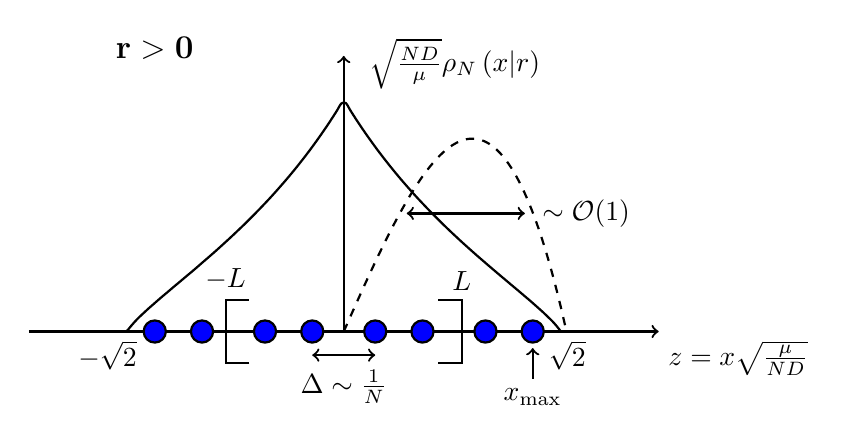
\begin{tikzpicture}[scale=2]

    % Draw the horizontal line representing the interval [-sqrt(2), sqrt(2)]
    \draw[thick, ->] (-2, 0) -- (2, 0);
    \draw[thick, ->] (0, 0) -- (0, 1.75);

    % Label the endpoints
    \node[below] at (-1.5, 0) {\(-\sqrt{2}\)};
    \node[below] at (1.42, 0) {\(\sqrt{2}\)};
    \node[right] at (0.1, 1.7) {$\sqrt{\frac{N D}{\mu}}\rho_N\left(x | r\right)$};
	\node[below right] at (2, 0) {$z = x \sqrt{\frac{\mu}{N D}}$};    
    
    \node at (-1.2, 1.8) {\large $\mathbf{r > 0}$};

    % Place some particles along the line
    \foreach \x in {-1.2, -0.9, -0.5, -0.2, 0.2, 0.5, 0.9, 1.2} {
        \fill[blue] (\x, 0) circle (2pt);
        \draw[black, thick] (\x, 0) circle (2pt);
    }

    % Draw the semi-circle density above
    \begin{scope}
        \clip (-1.414,0) rectangle (1.414,1.5);
        \draw[thick, domain=-1.41:1.41, samples=100, smooth] 
            plot ({\x}, {11/(6.28) * (1/sqrt(sqrt(2 - \x*\x)) - 6.4 * abs(\x) * acos(abs(\x)/1.414)/(360*sqrt(2 - \x*\x)*sqrt(sqrt(2 - \x*\x)) )});
    \end{scope}
    
    \begin{scope}
    	\clip (-1.414, 0) rectangle (1.414, 1.5);
    	\draw[thick, domain=0:1.41, samples=50, smooth, dashed] 
        	plot ({\x}, {2.25 * \x * (1 - \x*\x/2)});
    \end{scope}
    
    \draw[<->, thick] (0.4, 0.75) -- (1.15, 0.75);
    \node[right] at (1.2, 0.75) {$\sim \mathcal{O}(1)$};
    
 	\draw[thick] (-0.6, -0.2) -- (-0.75, -0.2) -- (-0.75, 0.2) -- (-0.6, 0.2);
    \draw[thick] (0.6, -0.2) -- (0.75, -0.2) -- (0.75, 0.2) -- (0.6, 0.2);

    % Labels for the box limits
    \node[above] at (-0.75, 0.2) {\(-L\)};
    \node[above] at (0.75, 0.2) {\(L\)};
    
    \draw[->, thick] (1.2, -0.3) node[below] {$x_{\rm max}$} -- (1.2, -3pt);
    
    \draw[<->, thick] (-0.2, -0.15) -- (0.2, -0.15);
    
    \node at (0, -0.35) {$\Delta \sim \frac{1}{N}$};

\end{tikzpicture}

\end{document}